\documentclass{article}
\usepackage{enumitem}
\usepackage{graphicx} % Package to handle images

% Title and Author
\title{19CSE302 - Design Analysis Of Algorithms \\ Lab Evaluation 1}
\author{Praneeth V - CB.EN.U4CSE22244 \\ Sai Krishna - CB.EN.U4CSE22246}

\begin{document}

\maketitle

\section*{Lab Evaluation Questions}

\begin{enumerate}
    \item Analysis of Sorting algorithms
    \begin{enumerate}[label*=\arabic*.]
      \item \textbf{In-Place Quick Sort (with last element as the pivot)}

        Quick sort applies the Divide-And-Conquer strategy to sort a subarray A[p..n]:


        \textbf{Divide} : The array is rearranged into two subarrays such that A[p .. q-1 ] is less than that of A[q] and the other subarray A[q+1 .. n] 
        greater than A[q]. Here A[q] is the pivot element.

        \textbf{Conquer} : We sort the subarrays A[p .. q-1] and A[q+1 .. n]

        \textbf{Combine}: Now, we combine the sorted arrays together. 

        The time complexity of the In-Place Quick Sort depends on whether the partitioning is balanced or not, and depends on which elements are used for partitioning. 

        If the partitioning is balanced: It's the best case where the algorithm runs as fast as merge sort. Since the partitioning is balanced, we get two even halves where one is of the size \( \lfloor n/2 \rfloor \) and the other one of the size \( \lfloor n/2 \rfloor - 1 \). So the recurrence relation for this becomes: \( T(n) = 2 T(n/2) + \Theta(n) \) and by Master's Theorem, it becomes \( T(n) = \Theta(n \log n) \). 

        If the partitioning is unbalanced: Its the worst case where we have one subarray with size of \( n-1 \) and the other subarray with the size of 0. The time complexity of the partitioning costs \( \Theta(n) \) time and the recurrence relation for this case becomes:
        \( T(n) = T(n - 1) + \Theta(n) \) and making the overall time complexity \( T(n) = \Theta(n^2) \) and this case mostly happens when the array is already sorted. 

        If the partitioning is based on proportionality: Its the average case where the partitioning is done based on some proportions where the partitioning is like x-to-\(10-x\), then in this case the recurrence relation becomes like: \( T(n) = T(x \cdot n/10) + T(n/10) + c \cdot n \) in which just reaching the depth of the recursion tree for partition takes \( \log_{10/x} n \) which is \( \Theta(\log n) \) and the cost at each level is \( n \) making the time complexity: \( T(n) = O(n \log n) \)

        The Space complexity for In-Place Quicksort is \( O(\log n) \) for best and average case partitioning where \( logn \) represents the size of the recursion tree and in the worst case partitioning the space complexity becomes \( O (n) \) as the recursion tree becomes skewed leading to the size of the tree to be equal to the number of elements in an array. 

        % Code Section 1.1.1
        \begin{verbatim}
        Test Case 1: For size 100:
        \end{verbatim}

        % Image Section 1.1.1
        \begin{figure}[h]
            \centering
            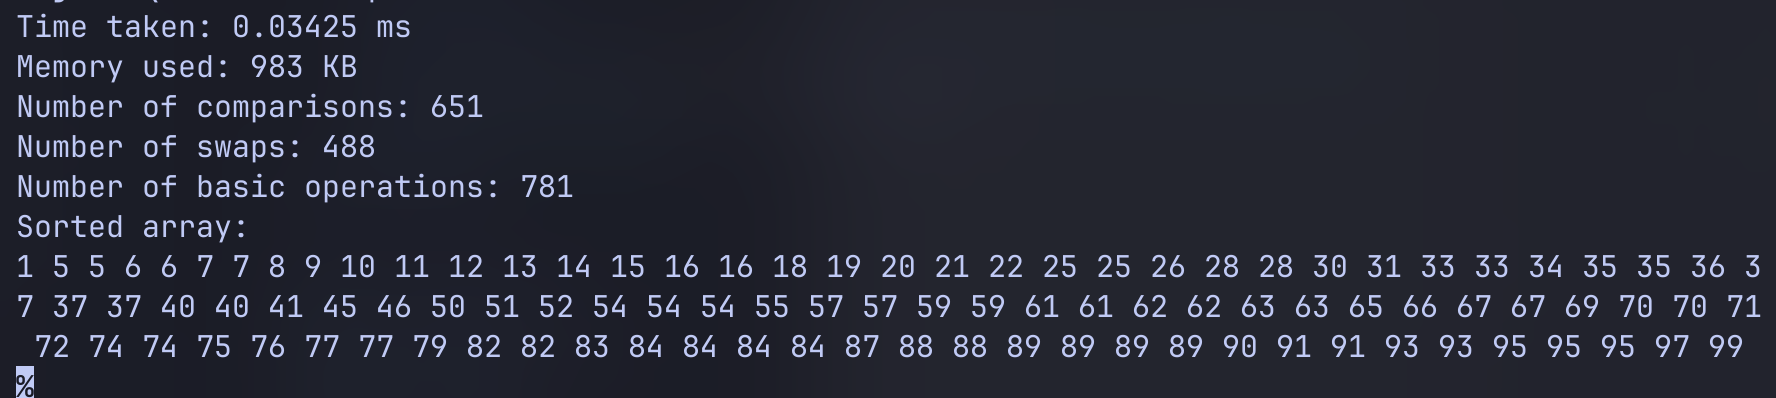
\includegraphics[width=0.8\textwidth]{./quicksort-tc-1.png}
            \label{fig:image1}
        \end{figure}

        % Code Section 1.1.2
        \begin{verbatim}
        Test case 2: For size 300
        \end{verbatim}

        % Image Section 1.1.2
        \begin{figure}[h]
            \centering
            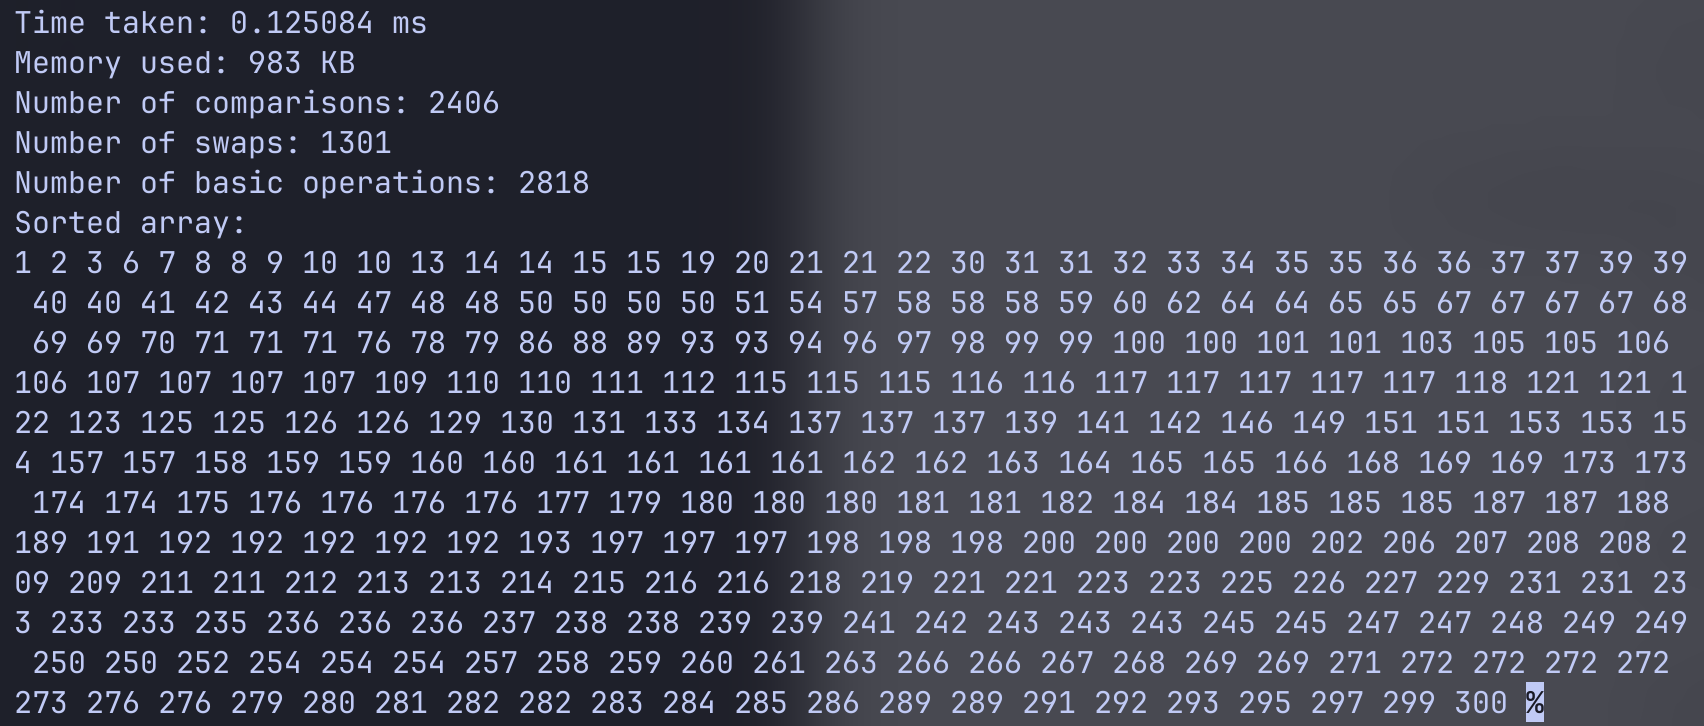
\includegraphics[width=0.8\textwidth]{./quicksort-tc-2.png}
            \label{fig:image2}
        \end{figure}

        % Code Section 1.1.3
        \begin{verbatim}
        Test case 3: For size 500
        \end{verbatim}

        % Image Section 1.1.3
        \begin{figure}[h]
            \centering
            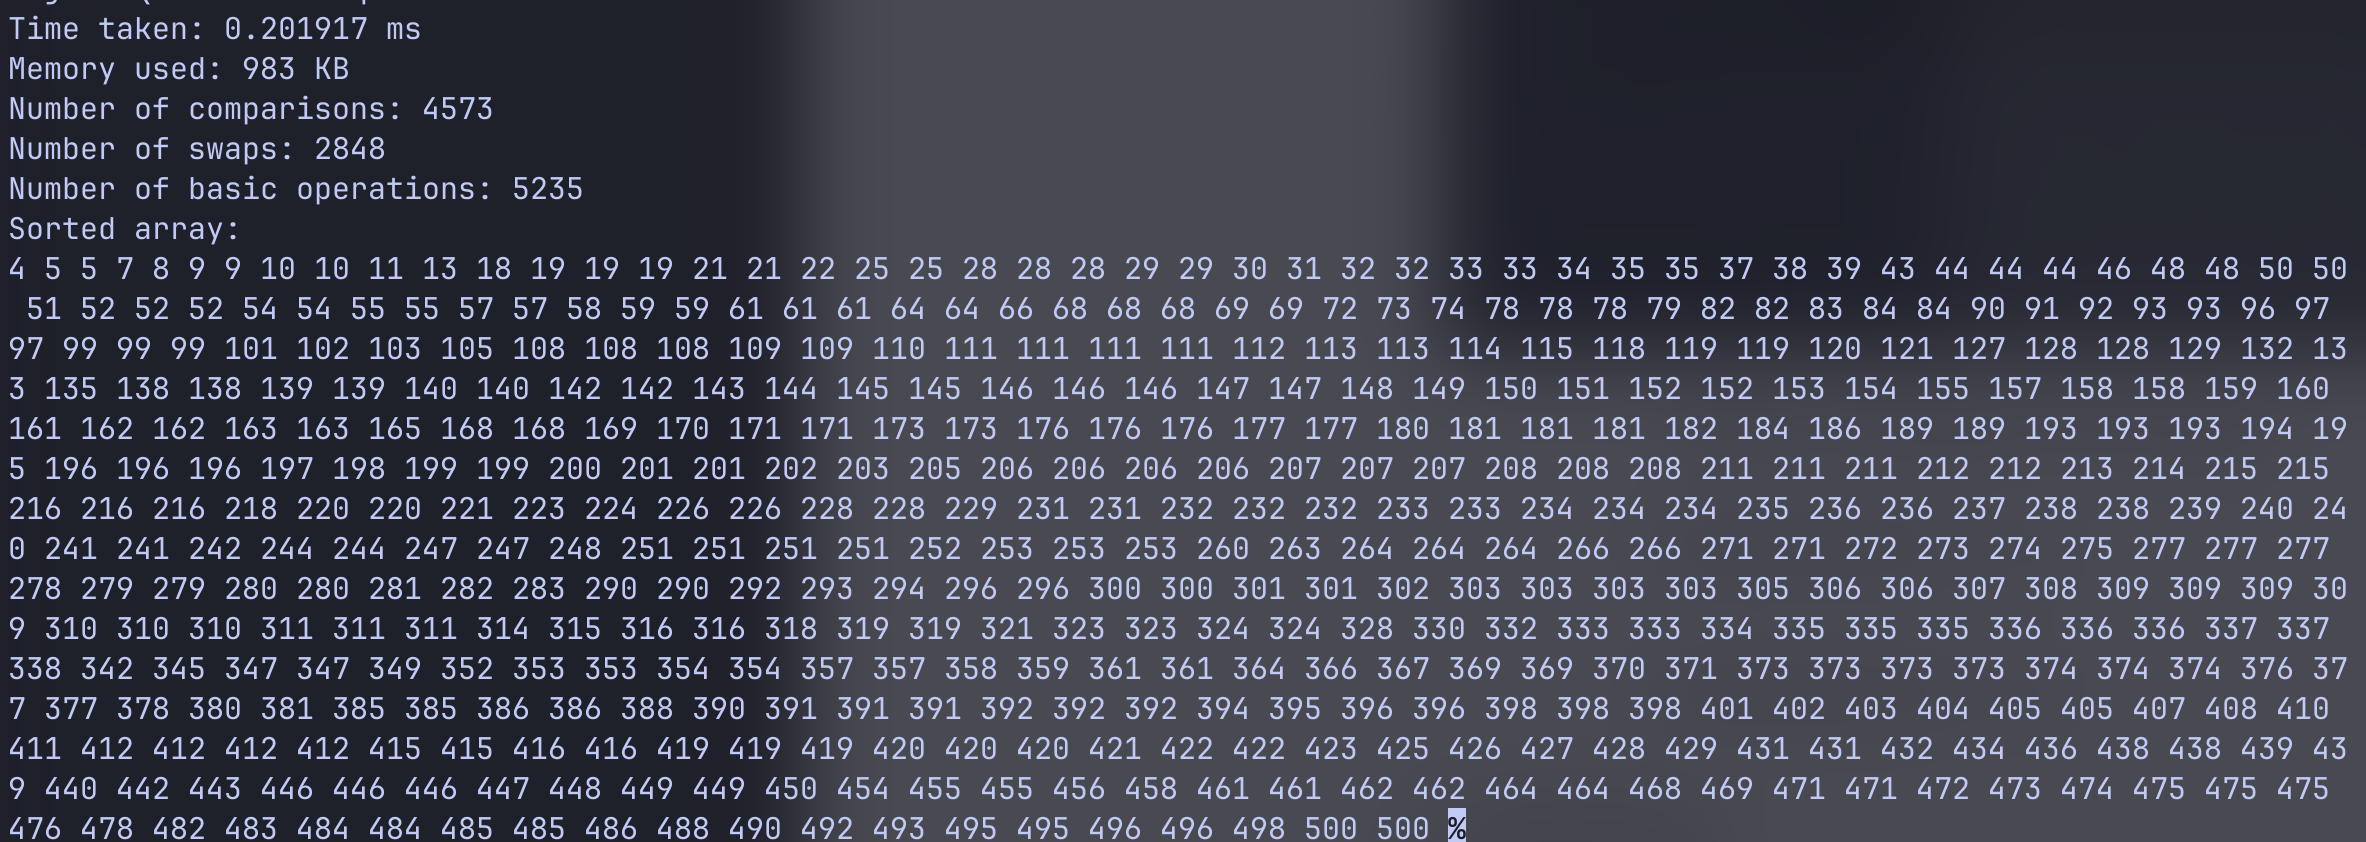
\includegraphics[width=0.8\textwidth]{./quicksort-tc-3.png}
            \label{fig:image3}
        \end{figure}

        % Code Section 1.1.4
        \begin{verbatim}
        Test case 4: For size 1000
        \end{verbatim}

        % Image Section 1.1.4
        \begin{figure}[h]
            \centering
            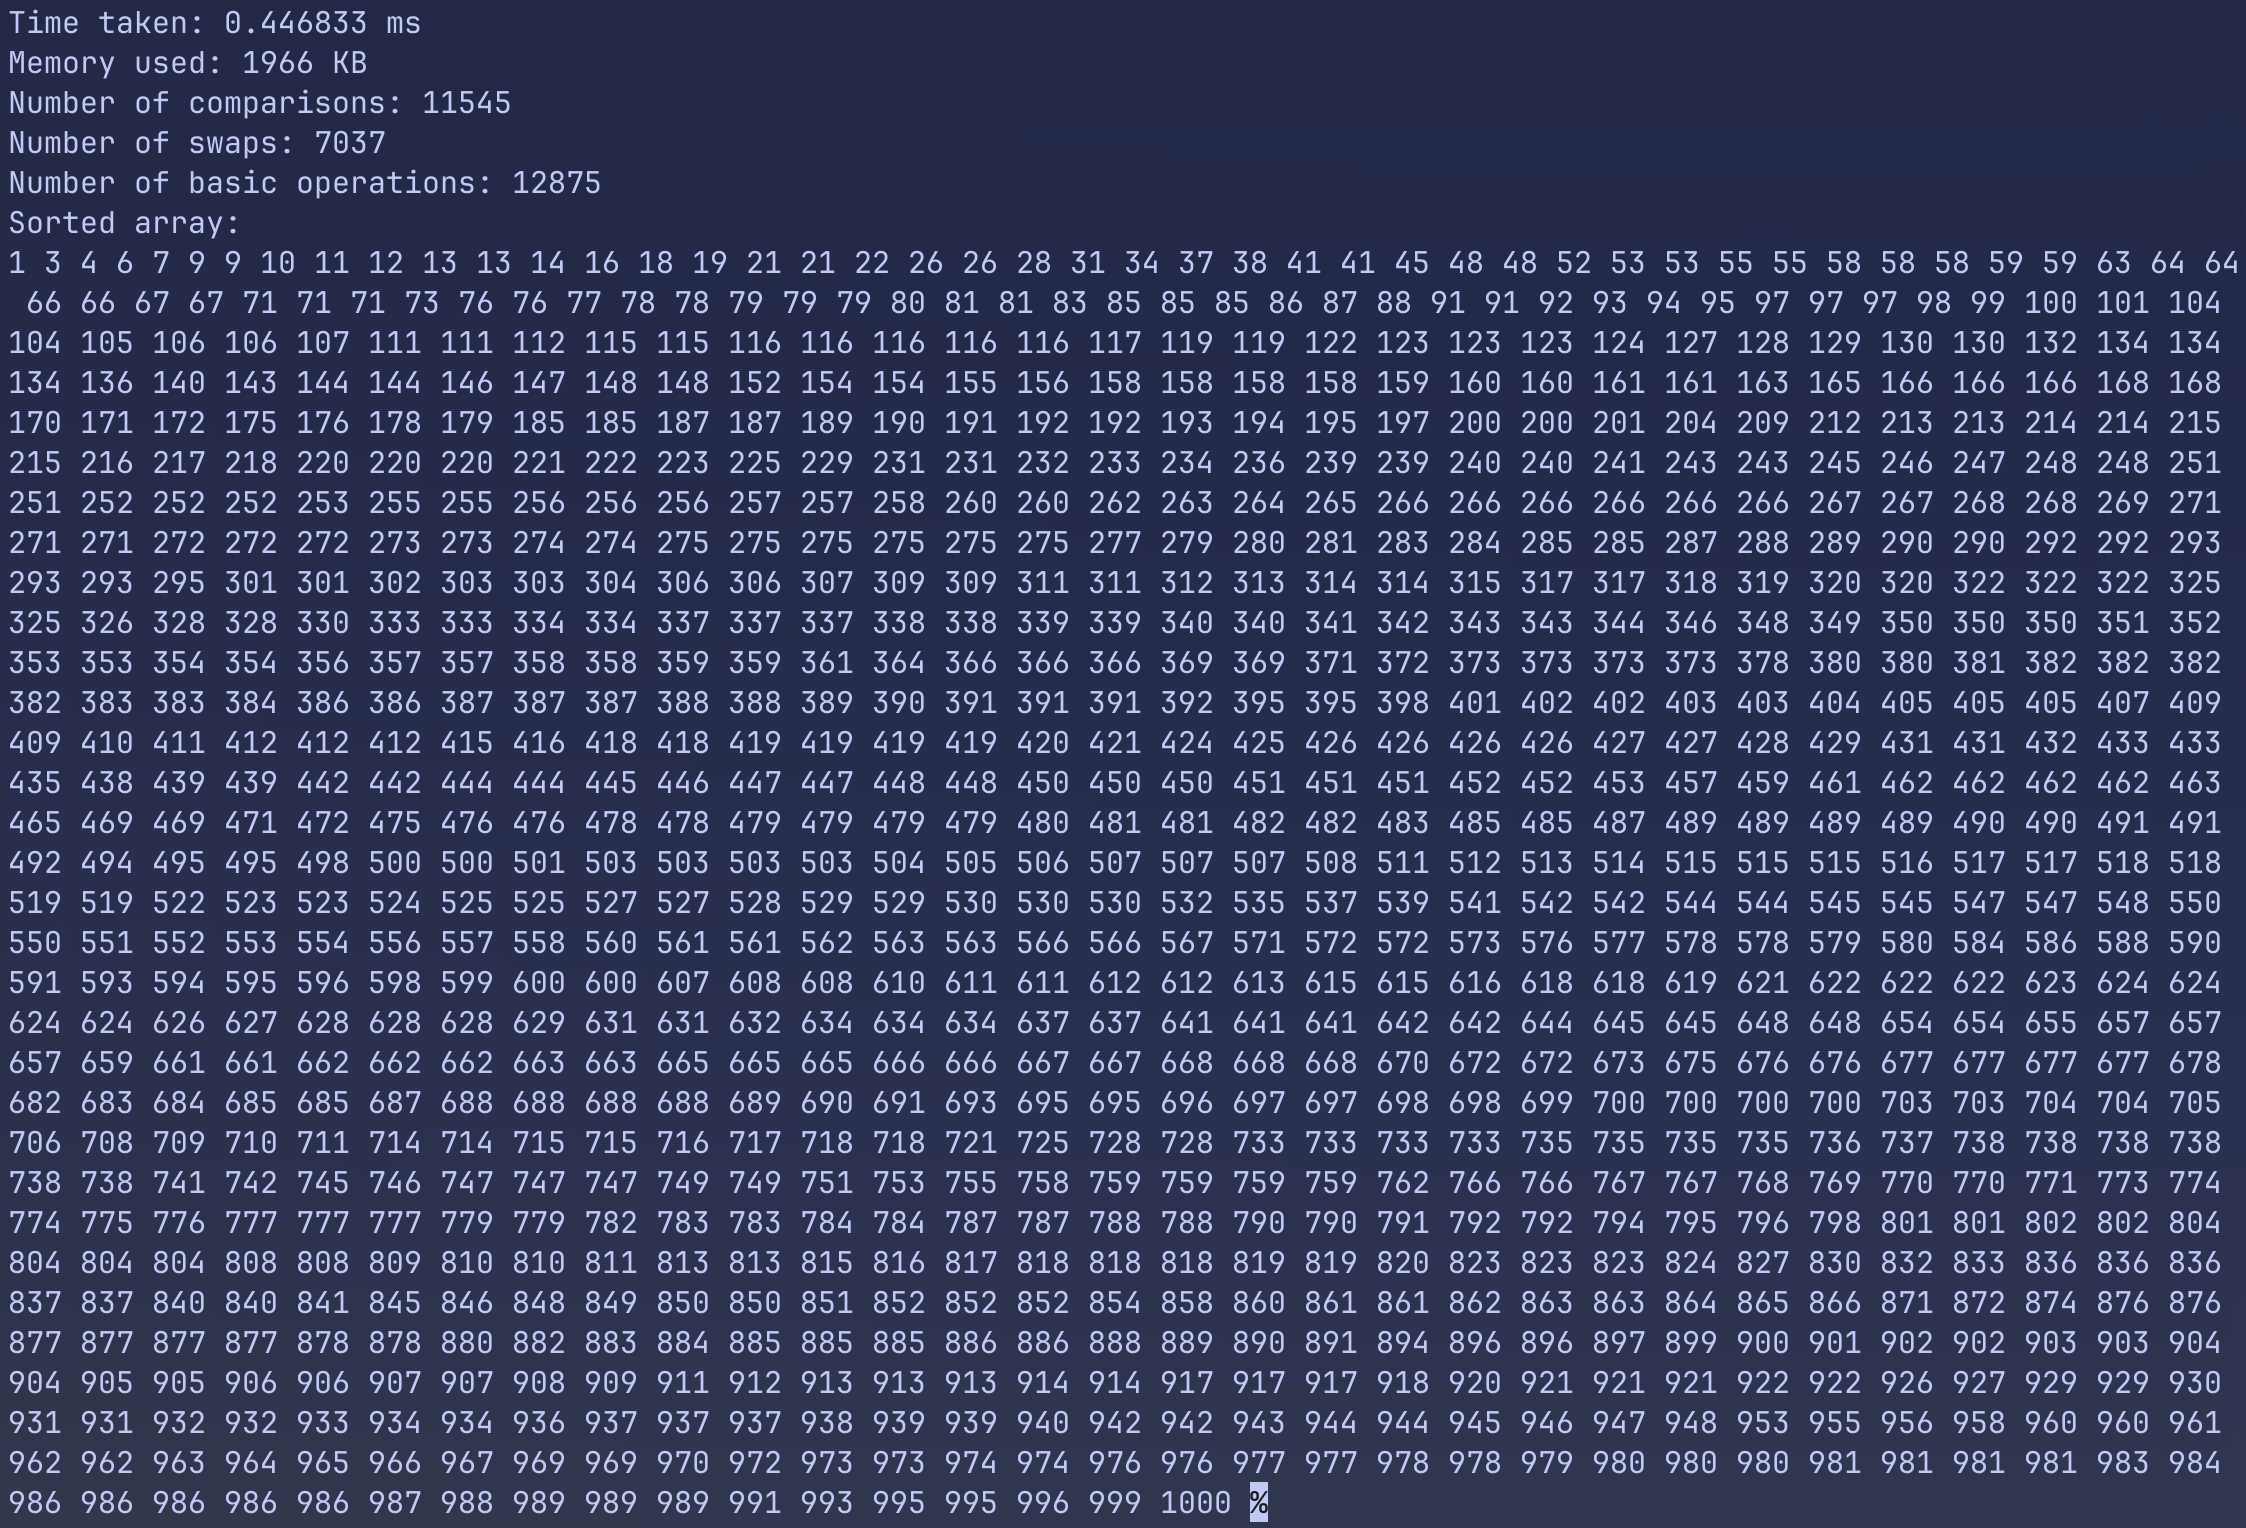
\includegraphics[width=0.8\textwidth]{./quicksort-tc-4.png}
            \label{fig:image4}
        \end{figure}

      \item \textbf{Three-way merge sort}

          Merge sort applies the Divide-And-Conquer strategy to sort an array A[p .. n]. Three-way merge sort again follows the Divide-and-Conquer paradigm where,

          \textbf{Divide} : Divide the array into three equal parts.

          \textbf{Conquer} : Recursively sort each of the three subarrays. 

          \textbf{Combine} : Merge the three sorted subarrays into one sorted array. 
          
          \textbf{Time complexity} : Let \( T(n) \) be the time complexity of sorting an array of size n. Since the array is being divided into three equal parts, each of size almost equal to \( n/3 \) and each part is sorted recursively. The merging of all the three parts will take an overall time complexity of \( O(n) \), so the recurrence relation for this sort is:
            
          \textbf{ Recurrence Relation: \(T(n) = 3T (n/3) + O(n) \) } 

          \textbf{ Time complexity: \( T(n) = O(n logn) \) }

        \textbf{ Space complexity } : Three-way merge sort needs extra space and this space is proprotional to the size of array being sorted where the recursion depth is \( O(log3 n) \) leading to an overall space complexity of \( O(n) \).

        % Code Section 1.2.1
        \begin{verbatim}
        % Code Section 1.2.1
        \end{verbatim}

        % Image Section 1.2.1
        \begin{figure}[h]
            \centering
            \includegraphics[width=0.8\textwidth]{path/to/image5.png}
            \caption{Description of the image}
            \label{fig:image5}
        \end{figure}

        % Code Section 1.2.2
        \begin{verbatim}
        % Code Section 1.2.2
        \end{verbatim}

        % Image Section 1.2.2
        \begin{figure}[h]
            \centering
            \includegraphics[width=0.8\textwidth]{path/to/image6.png}
            \caption{Description of the image}
            \label{fig:image6}
        \end{figure}

        % Code Section 1.2.3
        \begin{verbatim}
        % Code Section 1.2.3
        \end{verbatim}

        % Image Section 1.2.3
        \begin{figure}[h]
            \centering
            \includegraphics[width=0.8\textwidth]{path/to/image7.png}
            \caption{Description of the image}
            \label{fig:image7}
        \end{figure}

        % Code Section 1.2.4
        \begin{verbatim}
        % Code Section 1.2.4
        \end{verbatim}

        % Image Section 1.2.4
        \begin{figure}[h]
            \centering
            \includegraphics[width=0.8\textwidth]{path/to/image8.png}
            \caption{Description of the image}
            \label{fig:image8}
        \end{figure}

      \item \textbf{In-place Heap Sort}

          In-place Heap sort is a comparision based algorithm that uses a binary heap data structure to sort an array where the algorithm has two phases:

          \textbf{Heap Construction} : The input array is made into a max-heap. 

          \textbf{Sorting} : The heap being a max-heap, the largest element will be the root of the heap, the root element or the root node will be swapped with the last element of the heap, thereby reducing the size of the heap by one and then we have heapify the heap back since one element has been removed and this process is repreasted until the heap is reduced to a single element. 

          \textbf{Time complexity analysis : } Building the max heap from an unordered array taken \( O(n) \) time and moving down the right element down the heap will take the time complexity of \( O(log n) \) where \( logn \) is the size or the height of the heap. 

        \textbf{ Time complexity:} \( T(n) = O(n + logn) = O(n logn) \) .

          \textbf{ Space complexity:} Since the heap is being made from the array itself and we are not using any auxillary space while performing any operations like MAX-HEAPIFY or BUILD-MAX-HEAP, the space complexity is \( O(1) \).

        % Code Section 1.2.1
        \begin{verbatim}
        % Code Section 1.2.1
        \end{verbatim}

        % Image Section 1.2.1
        \begin{figure}[h]
            \centering
            \includegraphics[width=0.8\textwidth]{path/to/image5.png}
            \caption{Description of the image}
            \label{fig:image5}
        \end{figure}

        % Code Section 1.2.2
        \begin{verbatim}
        % Code Section 1.2.2
        \end{verbatim}

        % Image Section 1.2.2
        \begin{figure}[h]
            \centering
            \includegraphics[width=0.8\textwidth]{path/to/image6.png}
            \caption{Description of the image}
            \label{fig:image6}
        \end{figure}

        % Code Section 1.2.3
        \begin{verbatim}
        % Code Section 1.2.3
        \end{verbatim}

        % Image Section 1.2.3
        \begin{figure}[h]
            \centering
            \includegraphics[width=0.8\textwidth]{path/to/image7.png}
            \caption{Description of the image}
            \label{fig:image7}
        \end{figure}

        % Code Section 1.2.4
        \begin{verbatim}
        % Code Section 1.2.4
        \end{verbatim}

        % Image Section 1.2.4
        \begin{figure}[h]
            \centering
            \includegraphics[width=0.8\textwidth]{path/to/image8.png}
            \caption{Description of the image}
            \label{fig:image8}
        \end{figure}



      \item \textbf{Bucket Sort}

        Bucket sort assumes that the input is drawn from a uniform distribution and has the average-case running time of \( O(n) \) where the algorithm assumes that the input ranges within the interval \( [0, 1) \). In this technique we distribute the elements into buckets where they can be sorted using insertion sort or any other sorting technique for that matter and then the sorted elements are then gathered in an orderly manner.

          \textbf{Time complexity analysis : } Building the max heap from an unordered array taken \( O(n) \) time and moving down the right element down the heap will take the time complexity of \( O(log n) \) where \( logn \) is the size or the height of the heap. 

        \textbf{ Time complexity:} The time complexity for this algorithm depends on few cases:
        1. Best case complexity where there is no need for any sorting as the array is already sorted and this happens when the elements are uniormly distributed and the time complexity will be \( O(n+k) \) where \( O(n) \) is for making buckets and \( O(k) \) is for sorting the buckets with linear time at best case scenario. 

        2. Average case complexity where the elements are jumbled order that is not properly in a sorted manner but the elements are uniformly distributed making the average case time complexity to \( O(n+k) \). 

        3. Worst case complexity where all or majority of the elements are placed in such a way that distribution is very skewed or even placed in the same bucket making the time complexity \( O(n**2) \)

        \textbf{Space Complexity: } The space complexity is \( O(n * k) \) where n is the number of elementts in the input array that needs to be sorted and k is the the number of buckets used in the algorithm. 

        % Code Section 1.2.1
        \begin{verbatim}
        % Code Section 1.2.1
        \end{verbatim}

        % Image Section 1.2.1
        \begin{figure}[h]
            \centering
            \includegraphics[width=0.8\textwidth]{path/to/image5.png}
            \caption{Description of the image}
            \label{fig:image5}
        \end{figure}

        % Code Section 1.2.2
        \begin{verbatim}
        % Code Section 1.2.2
        \end{verbatim}

        % Image Section 1.2.2
        \begin{figure}[h]
            \centering
            \includegraphics[width=0.8\textwidth]{path/to/image6.png}
            \caption{Description of the image}
            \label{fig:image6}
        \end{figure}

        % Code Section 1.2.3
        \begin{verbatim}
        % Code Section 1.2.3
        \end{verbatim}

        % Image Section 1.2.3
        \begin{figure}[h]
            \centering
            \includegraphics[width=0.8\textwidth]{path/to/image7.png}
            \caption{Description of the image}
            \label{fig:image7}
        \end{figure}

        % Code Section 1.2.4
        \begin{verbatim}
        % Code Section 1.2.4
        \end{verbatim}

        % Image Section 1.2.4
        \begin{figure}[h]
            \centering
            \includegraphics[width=0.8\textwidth]{path/to/image8.png}
            \caption{Description of the image}
            \label{fig:image8}
        \end{figure}

       



      \item \textbf{Radix Sort}

        Radix sort is a sorting algorithm where we group the keys by their individual digits that share the same significant position and value. We take in a list of integers which are in base or some radix where k is the largest element in the list, then we perform counting sort on each single digit from least to most significant digit. 

        \textbf{Time complexity:} \( theta(d x (n + K)) \) where d is the number of digits in the largest element in the list that we will be sorting, since this sorting algorithm is basically repeating counting sort for the number of digits present in the max element of an array, the time complexity will become \( theta (d x (n+k )) \) where \( theta(n + k) \). 

        \textbf{Space complexity:} \( O(n + k) \) where n is the number of elements in the array and k is the  number of buckets that is dependent on the radix or the base, for eg. If we are taking in decimal numbers where the base is 10 then the vukets range from 0 to 9 and k = 10. So the space complexity accounts for the additional storage required for output array of size n and the size of the counting array which is size k.

        % Code Section 1.2.1
        \begin{verbatim}
        % Code Section 1.2.1
        \end{verbatim}

        % Image Section 1.2.1
        \begin{figure}[h]
            \centering
            \includegraphics[width=0.8\textwidth]{path/to/image5.png}
            \caption{Description of the image}
            \label{fig:image5}
        \end{figure}

        % Code Section 1.2.2
        \begin{verbatim}
        % Code Section 1.2.2
        \end{verbatim}

        % Image Section 1.2.2
        \begin{figure}[h]
            \centering
            \includegraphics[width=0.8\textwidth]{path/to/image6.png}
            \caption{Description of the image}
            \label{fig:image6}
        \end{figure}

        % Code Section 1.2.3
        \begin{verbatim}
        % Code Section 1.2.3
        \end{verbatim}

        % Image Section 1.2.3
        \begin{figure}[h]
            \centering
            \includegraphics[width=0.8\textwidth]{path/to/image7.png}
            \caption{Description of the image}
            \label{fig:image7}
        \end{figure}

        % Code Section 1.2.4
        \begin{verbatim}
        % Code Section 1.2.4
        \end{verbatim}

        % Image Section 1.2.4
        \begin{figure}[h]
            \centering
            \includegraphics[width=0.8\textwidth]{path/to/image8.png}
            \caption{Description of the image}
            \label{fig:image8}
        \end{figure}
\end{enumerate}

  \item Comparitive analysis on the effectiveness of an algorithm on the usage of a data structure
    \begin{enumerate}[label*=\arabic*.]
      \item \textbf{Binary Search} 

        Binary Search is a searching algorithm that searches for an element in a sorted array. It is a half-interval search algorithm where we compare the target value with that of the middle element. Depending on the comparision we shift our searching range in the sorted array.  

        This algorithm runs in \( O(logn) \) time complexity where n is the number of elements in the array and since we keep dividing the array in half to halven the area to search for, it makes the sarching go till the depth of \( O(logn) \) where \( logn \) is the height of that tree. 

        But the catch here being that, we have to use the sorted array for this algorithm to work, so from scratch for an unordered array, the time complexity at best will be \( O( nlogn + logn ) \) where \( O(nlogn) \) is the best time complexity for sorting the array and \( logn \) is for binary search and the worst being \( O(n**2 + logn) \).


      \item \textbf{Binary search using AVL Trees}

        Binary search using AVL tree is an efficient way to tackle the problem of sorting the array at first and then searching. In AVL tree, insertion of each element and then maintaining the balance of the tree takes \( O(logn) \) and since there are n elements in the array it will take \( O(nlogn) \) for inserting all the elemnts in the AVL tree while maintaining the AVL tree property. 

        Thereby we dont have to face the consequences of the worst-case scenario being \( O(n**2 + logn) \) where we maintain the time complexity \( O(nlogn + logn) \) for best, average, and worst time complexity thereby ensuring uniform but fast performance. 

        The only caveat of this approach is the space complexity as we will be using auxilarry space to store n elements from an array as nodes, the space complexity becomes \( O(n) \) compared to normal binary search where we do not use any auxillary space. 

    \end{enumerate}
\end{enumerate}




\end{document}

